\documentclass[../../note.tex]{subfiles}

% \usepackage[left=2.50cm, right=2.50cm, top=2.00cm, bottom=2.00cm]{geometry}

\begin{document}

\chapter{Theory of Electrodynamics}
%\title{《电动力学》\\
%	84个必背知识点}
%\author{佚名}
%\begin{document}
%	\maketitle
	\section{零、数学与物理常量基础公式}
	\begin{enumerate}
		\item 矢量叉乘公式
		\begin{align}
		a \times(b \times c)=b(a \cdot c)-c(a \cdot b)
		\end{align}
		[*请自行结合 $\nabla$ 的微分性与线性叠加,得到 $\nabla \times(a \times b), \nabla \times(\nabla \times a)$ 等]
		\item 关于 $\nabla$ 的相关公式 (推导用):
		\begin{align}
		\nabla \cdot\left(\frac{R}{R^3}\right)=4 \pi \delta(R) \quad \nabla f(r)=\frac{\partial f}{\partial r} \nabla r=\frac{\partial f}{\partial r} \hat{r}
		\end{align}
		\item 关于 $\nabla$ 积分的相关公式:
		\begin{align}
			& \int_{\mathrm{V}} \nabla \cdot {A} \mathrm{d} \tau=\oint_{\mathrm{S}} {A} \cdot \mathrm{d} {S} \quad \int_{\mathrm{V}} \nabla \psi \mathrm{d} \tau=\oint_{\mathrm{S}} \psi \mathrm{d} S \\
			& \int_{\mathrm{V}} \nabla \times {A} d \tau=\oint_{\mathrm{S}} \mathrm{d} {S} \times {A} \\
			& \int_{\mathrm{S}} \nabla \times {A} \cdot \mathrm{d} {S}=\oint_{\mathrm{c}} {A} \cdot \mathrm{d} {l} \quad \int_{\mathrm{S}} \mathrm{d} {S} \times \nabla \psi=\oint_{\mathrm{c}} \psi \mathrm{d} {l}
		\end{align}
		\item 物理常量基本公式
		\begin{align}
		\mu_0 \epsilon_0=\frac{1}{c^2}
		\end{align}
	\end{enumerate}

\section{麦克斯韦方程组}
\begin{enumerate}
	\item 电场及标量势,及 2 者关系
	\begin{align}
	E(r)=\frac{1}{4 \pi \epsilon_0} \int \frac{\rho\left(r^{\prime}\right)}{R^3} {R} d \tau^{\prime}=-\nabla \varphi \quad \varphi(r)=\frac{1}{4 \pi \epsilon_0} \int \frac{\rho\left(r^{\prime}\right)}{R} d \tau^{\prime}
	\end{align}
	\item 电偶极子 $(p=q l)$ 的电场及电势
	\begin{align}
	\varphi=\frac{1}{4 \pi \varepsilon_0} \frac{p \cdot r}{r^3} \quad E=-\frac{1}{4 \pi \varepsilon_0}\left[\frac{p-3(p \cdot \hat{r}) \hat{r}}{r^3}\right]
	\end{align}
	\item 电荷守恒/连续性方程:
	\begin{align}
	\frac{\partial \rho}{\partial t}+\nabla \cdot {j}=0 \quad {j}=\rho v
	\end{align}
	\item 磁场及矢势,及 2 者关系
	\begin{align}
	B=\frac{\mu_0}{4 \pi} \int \frac{j\left(r^{\prime}\right) d \tau^{\prime} \times R}{R^3}=\nabla \times A \quad A=\frac{\mu_0}{4 \pi} \int \frac{j\left(r^{\prime}\right)}{R} d \tau^{\prime}
	\end{align}
	\item 点电荷在电磁场中的受力
	\begin{align}
	{F}=q({E}+{v} \times {B})
	\end{align}
	\item 磁偶极子 $(m=I S)$ 的矢势及磁场
	\begin{align}
	A=\frac{\mu_0}{4 \pi} \frac{m \times r}{r^3} \quad B=-\frac{\mu_0}{4 \pi}\left[\frac{m-3(m \cdot \hat{r}) \hat{r}}{r^3}\right]
	\end{align}
	\item 真空及介质中的 Maxwell 方程组
	\begin{equation}
	\left\{\begin{array} { l } 
		{ \nabla \cdot  { E } = \rho / \epsilon _ { 0 } } \\
		{ \nabla \times  { E } = - \frac { \partial } { \partial t } B } \\
		{ \nabla \cdot  { B } = 0 } \\
		{ \nabla \times  { B } = \mu _ { 0 }  { j } + \mu _ { 0 } \epsilon _ { 0 } \frac { \partial } { \partial t }  { E } }
	\end{array} \quad \left\{\begin{array}{l}
		\nabla \cdot {D}=\rho_f \\
		\nabla \times {E}=-\frac{\partial}{\partial t} B \\
		\nabla \cdot {B}=0 \\
		\nabla \times {H}={j}_f+\frac{\partial}{\partial t} {D}
	\end{array}\right.\right.
\end{equation}
	\item 各项同性材料中的本构关系
	\begin{align}
		& D=\epsilon {E}, {H}={B} / \mu \text { (无色散) } \\
		& D_\omega(r)=\epsilon(\omega) {E}_\omega(r), B_\omega(r)=\mu(\omega) {H}_\omega(r) \text { (色散介质) } \\
		& \left(j_\omega=\sigma(\omega) {E}_\omega\right)
	\end{align}
	\item 材料的线性响应
	\begin{align}
		{P}=\epsilon_0 \chi_e {E}, \quad \epsilon=\epsilon_r \epsilon_0=\left(1+\chi_e\right) \epsilon_0 \\
		M=\frac{1}{\mu_0} \frac{\chi_m}{1+\chi_m} {B}, \quad \mu=\mu_r \mu_0=\left(1+\chi_m\right) \mu_0,
	\end{align}
	\item 介质中的电荷和电流 (自由、极化、磁化)
\begin{align}
		\rho=\rho_f+\rho_p, \rho_p=-\nabla \cdot {P} \\
		{j}={j}_f+{j}_m+{j}_\rho, {j}_m=\nabla \times {M}, {j}_p=\frac{\partial {P}}{\partial t}
\end{align}
	\item 麦克斯韦方程组的边界条件 $(\nabla \rightarrow n)$
	\begin{equation}
	\left\{\begin{array}{l}
		n \cdot\left(D_1-D_2\right)=\sigma_f \text { 自由电荷面密度 } \\
		n \times\left(E_1-E_2\right)=0 \\
		n \cdot\left(B_1-B_2\right)=0 \\
		n \times\left(H_1-H_2\right)=\alpha_f \text { 面电流密度 }
	\end{array}\right.
\end{equation}
\end{enumerate}


\section{电磁场的守恒定律和对称性}
\begin{enumerate}
	\item 电 (磁) 场对电荷做功:
		\begin{align}
	d R={E} \cdot \mathrm{j} \mathrm{d} \tau \mathrm{d} t
\end{align}
	\item 真空中电磁场的能量守恒定律及各项的含义
	\begin{align}
		\frac{\mathrm{d}}{\mathrm{d} t}\left[W_m+\int u \mathrm{~d} \tau\right]=-\oint S_p \cdot \mathrm{d} {S} \\
		u(r, t)=\frac{1}{2}\left(\epsilon_0 E^2+\frac{1}{\mu_0} B^2\right), \quad S_p(r, t)=\frac{1}{\mu_0} {E} \times {B}
	\end{align}
	其物理意义为: 在一个闭合空间内物理量 (总能) $W_m+\int u \mathrm{~d} \tau$ 的增加等于从 边界流入闭合空间的 $S_p$ 的大小。其中 $u(r, t)$ 是 $r$ 点处 $t$ 时刻电磁场的能量密 度, $S_p$ 即为相应的能流密度,也称做坡印廷矢量。
	\item 真空中电磁场的动量守恒定律及各项的含义
\begin{equation}
	\frac{\mathrm{d} {G}_m}{\mathrm{~d} t}=-\oint \mathrm{d} {S} \cdot \overrightarrow{\vec{T}}-\frac{\mathrm{d}}{\mathrm{d} t} \int {g} \mathrm{d} \tau
\end{equation}
\begin{equation}
	\text { 电磁场的动量密度 } g=\epsilon_0(E \times B)=\frac{1}{c^2} S_p
\end{equation}
\begin{equation}
	\text { 动量流密度 } \overrightarrow{\vec{T}}=\frac{1}{2}\left(\epsilon_0 E^2+\frac{1}{\mu_0} B^2\right)-\epsilon_0 {E} {E}-\frac{1}{\mu_0} {B} {B}
\end{equation}
\begin{equation}
	\text { 受力 } {F}_m=\frac{\mathrm{d} {G}_m}{\mathrm{~d} t}
\end{equation}
	\item 带电的运动粒子在外磁场中的总动量
	\begin{align}
	p=m {v}+q {A}
\end{align}
	\item 介质中的电磁能量守恒定律
\begin{align}
	u(r, t)=\frac{1}{2}\left(\epsilon E^2+\mu H^2\right), \quad {S}_p({r}, t)={E} \times {H}
\end{align}
	\item 介质中电磁场的动量守恒定律
\begin{align}
	g^{\prime}=D \times B, \quad \overrightarrow{\overrightarrow{T}}=\frac{1}{2}(E \cdot D+B \cdot H) \overrightarrow{\overrightarrow{I}}-D E-B H
\end{align}
	
\end{enumerate}


\section{导体静电学}
\begin{enumerate}
	\item 导体静电问题中电势满足的方程及边界条件
	\begin{align}\left\{
		\begin{array}{l}
				\nabla^2 \varphi=-\rho / \epsilon \\
			\varphi \text { 在边界有限 } \\
			\left.\frac{\partial \varphi}{\partial n}\right|_{\text {边界 }}=-\frac{\sigma}{\epsilon}, \quad Q=-\epsilon \oint \frac{\partial \varphi}{\partial n} \mathrm{~d} S
		\end{array}
	\right.
\end{align}
	\item 格林互易定理
	给定一个有 $m$ 个导体组成的体系,假设当导体上的电荷为 $q_1, q_2, \cdots$ 时,它们 的电势等于 $\phi_i$ ,而对应另外一种电荷分布 $q_i^{\prime}$, 导体的电势分布为 $\phi_i^{\prime}$ ,那么有关 系式 $\sum_i q_i \phi_i^{\prime}=\sum_i q_i^{\prime} \phi_i$.
	\item 导体系中的总能和相互作用能
	\begin{align}
\text { 总能 } W=\frac{1}{2} \int \varphi \rho \mathrm{d} \tau=\frac{1}{2} \sum_i \phi_i Q_i
	\end{align}
	\begin{align}
\text { 相互作用能 } W=\frac{1}{2} \sum_i q_i \phi_i^{\prime}, \quad \phi_i^{\prime}=\sum_{j \neq i} \phi_j \text { 为其余电荷在 } q_i \text { 处电势 }
\end{align}
	\item 电容的定义
	\begin{align}
	q_i=\sum_j C_{i j} \phi_j, \phi_i=\sum_j C_{i j}^{-1} q_j \rightarrow W=\frac{1}{2} \sum_{i, j} C_{i j} \phi_i \phi_j
\end{align}
	\item 静电体系的稳定性一汤姆逊定理和恩肖定理
	
	汤姆逊定理:若导体系中每个导体的位置固定不变,电荷可再分布,则体系基 态对应,电荷的分布使所有导体均为等势体。
	
	恩肖定理:静电体系的平衡条件是体系中任一导体所处的位置的电场均为 0 , 因此无约束下静电体系没有平衡态。
	
	\item 导体表面所受静电力
	\begin{align}
	F_s=\frac{\epsilon_0}{2} E^2 \hat{e}_n=\frac{1}{2 \epsilon_0} \sigma^2 \hat{e}_n
	\end{align}
\end{enumerate}
\section{电介质静电学}
\begin{enumerate}
	\item 电介质的边界条件
	\begin{align}\left\{
		\begin{array}{l}
		\varphi_1=\varphi_2 \\
		\epsilon_1 \cdot \frac{\partial \varphi_1}{\partial n}-\epsilon_2 \cdot \frac{\partial \varphi_2}{\partial n}=-\sigma_f(\vec{n}: 2 \rightarrow 1)
			\end{array}
		\right.
\end{align}
	\item 唯一性定理
	对于确定的静电 (磁) 问题 (已知电荷分布和电介质分布 $\rho(r), \epsilon(r)$ 或电流和磁 介质分布),边条唯一决定解 (前提: 介质中 D 与 $E(H$ 与 $A)$ 之间的本构关系 为单调单值)
	\item 镜像法 (会做)
	
	%\begin{figure}[H]
	%	\centering
	%	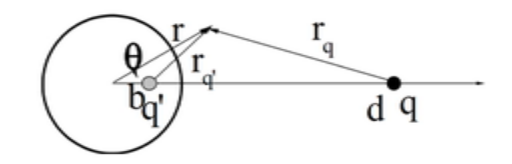
\includegraphics[width=0.4\linewidth]{../figures/fig1.png}
	%\end{figure}
	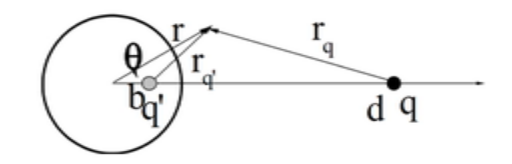
\includegraphics[scale = 0.3]{../figures/fig1.png}
	
	 \begin{align}
	q^{\prime}=\frac{R}{d} q, \quad b=\frac{R^2}{d}
	\end{align}
	
	\item 本征函数展开法
	
	外场为均匀电场时,对于球/柱体系,解只具有 $l=1$ 的项。
	
	\begin{align}\text{轴对称球坐标系} \varphi=\left(A r+\frac{B}{r^2}\right) \cos \theta\end{align}
	
\begin{align}
\text { 与 } \mathrm{z} \text { 无关的柱对称 } \varphi=B_0 \ln \rho+\left(A_1 \rho+B_1 \rho^{-1}\right) \cos \phi+\left(C_1 \rho+D_1 \rho^{-1}\right) \sin \phi
\end{align}
		\item 退极场
	\begin{align}
	{E}_d={E}_0-{E}_{\text {in }}=-L \cdot {P} / \epsilon_0
	\end{align}
	$L$ 为退极因子,取决于物体形状,对于球 $L=1 / 3$.
		\item 多极矩展开
\begin{align}
		\varphi=\frac{Q}{4 \pi \epsilon_0 r}-\frac{P}{4 \pi \epsilon_0} \nabla \frac{1}{r}+\frac{1}{4 \pi \epsilon_0} \frac{1}{6} \overrightarrow{\vec{D}}: \nabla \nabla \frac{1}{r} \\
		Q=\int \rho\left(r^{\prime}\right) \mathrm{d} \tau^{\prime}, {P}=\int \rho\left(r^{\prime}\right) r^{\prime} \mathrm{d} \tau^{\prime}, \overrightarrow{\vec{D}}=3 \int \rho\left(r^{\prime}\right) {r}^{\prime} {r}^{\prime} \mathrm{d} \tau^{\prime}
\end{align}
		\item 多极矩在外场中的作用
	\begin{align}
	W=Q \varphi-p \cdot {E}+\frac{1}{6} \overrightarrow{\vec{D}}: \nabla {E}
	\end{align}
		\item 电偶极矩在外场中的受力与力矩
	\begin{align}
	{F}_e=p \cdot \nabla {E}, \quad {M}=p \times {E}
	\end{align}
	
\end{enumerate}


	\section{静磁场}
\begin{enumerate}
	\item 磁场的矢势方程及边界条件
	\begin{align}
		& \nabla^2 A=-\mu_0 j \\
		& \hat{e}_n \times\left(A_1-A_2\right)=0 \\
		& \hat{e}_n \times\left[\frac{1}{\mu_1}\left(\nabla \times A_1\right)-\frac{1}{\mu_2}\left(\nabla \times A_2\right)\right]=\alpha_f
	\end{align}
	\item 静磁场总能
\begin{align}
	U_m=\frac{1}{2} \int {B} \cdot {H} \mathrm{d} \tau=\frac{1}{2} \int {A} \cdot {j} \mathrm{d} \tau
\end{align}
	\item 磁场的标量势解法中磁标势的定义,引入磁标势的条件及其意义
\begin{align}
	{H}=-\nabla \varphi_m
\end{align}
	
	1) 无传导电流;2) 引入磁壳使得空间为单连通;
	
	从而保证了 $\mathrm{H}$ 是个保守场,且保证了磁标势单值性.
	
	\item 磁介质中的边界条件
	\begin{align}
	\left\{\begin{array}{l}
		\varphi_1=\varphi_2 \\
		\mu_1 \cdot \frac{\partial \varphi_1}{\partial n}=\mu_2 \cdot \frac{\partial \varphi_2}{\partial n}
	\end{array}\right.
	\end{align}
	\item 铁磁介质中的边界条件 (饱和磁化为 $\left.M_0^i\right)$
	\begin{align}
	\left\{\begin{array}{l}
		\varphi_1=\varphi_2 \\
		\frac{\partial \varphi_1}{\partial n}-\frac{\partial \varphi_2}{\partial n}=e_n \cdot\left(M_0^1-M_0^2\right)
	\end{array}\right.
	\end{align}
	\item 磁多极展开
	\begin{align}
	A=A^{(1)}=\frac{\mu_0}{4 \pi} \frac{m \times r}{r^3}, m=\frac{1}{2} \int r^{\prime} \times j \mathrm{~d} \tau^{\prime}
	\end{align}
	\item 磁偶极子的能量、受力和力矩
	\begin{align}
	U=-m \cdot B ; F=\nabla(m \cdot B) ; \tau=m \times B
		\end{align}
\end{enumerate}


\section{似稳场 (准静)}
\begin{enumerate}
	\item 似稳条件
	\begin{enumerate}
		\item 电磁场变化频率远小于金属特征频率 $\omega<<\omega_\sigma=\sigma_c / \epsilon$, 其中 ${j}=\sigma_c {E}$.
		\item  $R<<\lambda / 2 \pi$ 从而忽略位移电流与辐射	
	\end{enumerate}
	\item 似稳场方程
	\begin{align}
	\frac{\partial}{\partial t}\left(\begin{array}{l}
		{H} \\
		{E}
	\end{array}\right)=\frac{1}{\mu \sigma_c} \nabla^2\left(\begin{array}{l}
		{H} \\
		{E}
	\end{array}\right)
\end{align}
	\item 趋肤效应与趋肤深度
	\begin{align}
		{E}=\hat{x} A \exp [p z-i \omega t]=\hat{x} E_0 e^{-\alpha z} \cos (\omega t-\alpha z) 	\end{align}
		\begin{align}
		\delta=\frac{1}{\alpha}=\sqrt{\frac{2}{\mu \omega \sigma_c}}
	\end{align}
\end{enumerate}

\section{电磁波的传播}
\begin{enumerate}
	\item 电磁波的传播方程
	\begin{align}
	\left(\nabla^2-\epsilon \mu \frac{\partial}{\partial t^2}\right)\left(\begin{array}{l}
		E \\
		B
	\end{array}\right)=0
	\end{align}
	[* 请自行从 Maxwell 方程推导得到该式.]
		\item 电磁波的解
	\begin{align}
		E(r, t) & ={E}_0 \cos (k \cdot r-\omega t+\phi) \\
		B(r, t) & =B_0 \cos (k \cdot r-\omega t+\phi)
	\end{align}
		\item 电磁波的色散关系、波速、波长和折射率
	\begin{align}
		k^2=\epsilon \mu \omega^2 \\
		v^2=\frac{1}{\epsilon \mu}, v_p=\omega / k \\
		k=2 \pi / \lambda \\
		n=\sqrt{\epsilon_r \mu_r}=k \omega / c
	\end{align}
	
	\item 波矢与电场、磁场的关系
	\begin{align}
		k \cdot {E}_0 & =0, \quad k \cdot B_0=0 \\
		k \times {E}_0=\omega {B}_0, \quad k & \times B_0=-\epsilon \mu \omega {E}_0
	\end{align}
	\item 阻抗的定义
	\begin{align}
	Z=\sqrt{\mu / \epsilon},\left|{E}_0\right|=Z\left|{H}_0\right|
\end{align}
	\item 电磁波的能流
	\begin{align}
		\left\langle{S}_p\right\rangle=\frac{1}{2} \operatorname{Re}\left({E} \times {H}^*\right)=\frac{1}{2 Z} E_0^2 \hat{k}=\langle{u}\rangle \cdot {v} \\
		\langle{u}\rangle=\frac{\epsilon}{2} E_0^2
	\end{align}
	\item $E_0=\hat{x} E_{x 0} e^{i \phi_x}+\hat{y} E_{y 0} e^{i \phi_y}$ 的线偏振和圆偏振条件
	
	
	线偏振: $\phi_x=\phi_y$;
	
	圆偏振 $\phi_x-\phi_y= \pm \pi / 2,\left|E_{x 0}=E_{y 0}\right|$, 正负对应右旋、左旋偏振 $\hat{e}_{\text {right }}=(\hat{x}-i \hat{y}) / \sqrt{2}, \hat{e}_{\text {eft }}=(\hat{x}+i \hat{y}) / \sqrt{2}$
	
	\item 金属的有效电导率一—Drude 模型及其推导
	
	利用散射力模型 (平均 $\tau$ 时间受到一次异种粒子的散射而丟失所有的动量)
	\begin{align}
	\sigma(\omega)=\frac{n_e e^2}{m(-i \omega+1 / \tau)}
	\end{align}
	\item 金属的有效介电函数及其不同频段的行为
	\begin{align}
	\epsilon(\omega)=\epsilon_0 \epsilon_v+i \frac{\sigma(\omega)}{\omega}, \epsilon_r=\epsilon_v-\frac{\omega_p^2}{\omega(\omega+i / \tau)}, \quad \epsilon_v \approx 1
	\end{align}
	\begin{align}
	\epsilon_r(\omega) \approx \begin{cases}i \frac{\sigma_c}{\epsilon_0 \omega}, & \leq \mathrm{GHz} \\ 1-\left(\frac{\omega_p}{\omega}\right)^2, & \text { 可见光波段 }\end{cases}
	\end{align}
	在可见光波段,电子高频下碰撞时间远大于周期,几平不表现出损耗。在 $\mathrm{GHz}$ 波段,电子平均碰撞时间远小于电场周期,表现为欧姆损耗直流良导体特征。
	\item 等离共振频率及其物理含义
	\begin{align}
	\omega_p=\sqrt{\frac{n_e e^2}{\epsilon_0 m}}
	\end{align}
	表示自由电子气在外场的驱动下集体震荡。

	\item 导电介质的色散关系
	\begin{align}
	k^2=\left(\frac{\omega}{c}\right)^2 \epsilon_r(\omega)
	\end{align}
	\item 良导体在不同电磁波频率的行为
	\begin{enumerate}
		\item 在 $\mathrm{GHz}$ 以下, $1 / \omega>>\tau$ 既震荡又衰减,电磁场有 $\pi / 4$ 相位差, $\alpha=\sqrt{\sigma_c \mu_0 \omega / 2}$, 趋肤深度 $\delta=\alpha^{-1}$.
		\item  在光波段 $k^2=\left(\omega^2-\omega_p^2\right) / c^2$ ,电磁场 $\pi / 2$ 相位差. 当
		
		$\omega<\omega_p$ ,不传播,造成反射;
		
		当 $\omega=\omega_p$ 隧穿至极值;
		
		当 $\omega>\omega_p$ ,紫外透明,有一定反射.
	\end{enumerate}
	\item 非良导体在不同电磁波频率的行为
	
	非良导体 $\omega \ll 1 / \tau$, 电磁场几平无相位差,电磁波传播伴随很小的衰减。
	
	\item 各向异性介质/旋光介质中的本构关系
	\begin{align}
		{D}_\omega=\epsilon_0 \vec{\epsilon}_r(\omega) {E} . \\
		\overrightarrow{\vec{\epsilon}}_r(\omega)=\left(\begin{array}{ccc}
			\epsilon_1 & i \epsilon_2 & 0 \\
			-i \epsilon_2 & \epsilon_1 & 0 \\
			0 & 0 & \epsilon_3
		\end{array}\right) \\
		\epsilon_1=1-\frac{\omega_p^2}{\omega^2-\omega_B^2}, \epsilon_2=\frac{\omega_p^2 \omega_B}{\left(\omega^2-\omega_B^2\right) \omega}, \epsilon_3=1-\frac{\omega_p^2}{\omega^2}, \omega_B=-\frac{e B_0}{m}
	\end{align}
	\item 左 $\left(k_{-}\right)$右 $\left(k_{+}\right)$旋光的色散关系
		\begin{align}
	k_{ \pm}=\frac{\omega}{c} \sqrt{\epsilon_1 \pm \epsilon_2}
	\end{align}
	\item 法拉第效应
	
	与入射光比较偏振方向旋转了如下的角度 $\Delta \phi=\left(k_{+}-k_{-}\right) \cdot d / 2$.
	\item 电磁波在介质界面反射、折射的基本规律及其物理本质
	\begin{enumerate}
	%	\begin{figure}[H]
	%		\centering
	%		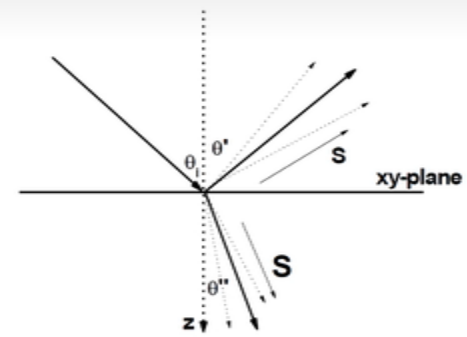
\includegraphics[width=0.4\linewidth]{../figures/fig2.png}
	%	\end{figure}
    
		\item 反射波、折射波与入射波 $\omega$ 相等一一时间平移不变性
		
		\item 入射线、反射线和折射线在同一平面内, $k_{\|}$相同一一空间平移不变性
		
		\item 在正常介质中, 反射波 $k_z^{\prime}$ 应取负根,折射波 $k_z^{\prime \prime}$ 应取正根一一因果律 
		\item 入射角等于反射角―一空间平移不变性
		
		\item Snell law ―空间平移不变性\begin{align}
		\frac{\sin \theta}{\sin \theta^{\prime \prime}}=\frac{k^{\prime \prime}}{k}=\frac{n_2}{n_1}
		\end{align}
		
		
	\end{enumerate}
    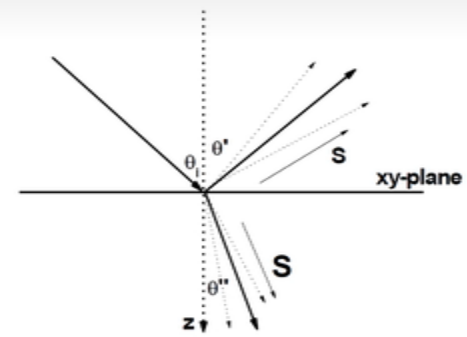
\includegraphics[scale = 0.6]{../figures/fig2.png}
	\item 电磁波在介质界面反射、折射的振幅关系
	\begin{enumerate}
		\item 横电波 $\mathrm{S} / \mathrm{TE}$ ,电场垂直于入射面,有效阻抗 $Z_{e f f}=Z / \cos \theta$
	\begin{align}
		E_0^{\prime}=\frac{Z_{e f f, 2}-Z_{e f f, 1}}{Z_{e f f, 2}+Z_{e f f, 1}} E_0=r_s \cdot E_0, E_0^{\prime \prime}=\frac{2 Z_{e f f, 2}}{Z_{e f f, 2}+Z_{e f f, 1}} E_0=t_s \cdot E_0
	\end{align}
		\item 横磁波 P/TM,磁场垂直于入射面, $Z_{\text {eff }}=Z \cos \theta$
		\begin{align}
		H_0^{\prime}=\frac{Z_{e f f, 1}-Z_{e f f, 2}}{Z_{e f f, 2}+Z_{e f f, 1}} H_0=r_p \cdot H_0, H_0^{\prime \prime}=\frac{2 Z_{e f f, 1}}{Z_{e f f, 2}+Z_{e f f, 1}} H_0=t_p \cdot H_0
	\end{align}
	\end{enumerate}
	\item 电磁波的反射率 $R$ 与透射率 $T$
	\begin{align}
	R=|r|^2, T=\left\{\begin{array}{l}
		\left|t_s\right|^2 \frac{Z_{e f f, 1}}{Z_{2 f f, 2}} \\
		\left|t_p\right|^2 \frac{Z_{e f f, 2}}{Z_{e f, 1}}
	\end{array}\right.
	\end{align}
	\item 布鲁斯特 Brewster 角及其意义
	
	当反射波与折射波相互垂直时, $P$ 偏振的电磁波完全不被反射, 入射角
\begin{align}
	\theta_B=\arctan \left(n_2 / n_1\right)
\end{align}
	\item 全反射临界角
\begin{align}
	\theta_C=\arcsin \left(n_2 / n_1\right)
\end{align}



\end{enumerate}


\section{波导和谐振腔}
\begin{enumerate}
	\item 波导管 (PEC) 的边界条件
	\begin{align}
		n \cdot B=0, n \times E=0 \\
		n \cdot D=\sigma, n \times H=j
	\end{align}
	\item 波导管中波的模式 (偏振)
	\begin{enumerate}
		\item 横电波 TE: $B_{0 z} \neq 0, E_{0 z}=0$
		\item 横电波 TM: $B_{0 z}=0, E_{0 z} \neq 0$
	\end{enumerate}
	
	\item TE 波的解及基模
	
	\begin{align}
	B_{0 z}=B_0 \cos \left(\frac{m \pi}{a} x\right) \cos \left(\frac{n \pi}{b} y\right) ; B_z=B_{0 z} \exp \left[i k_z z-\omega t\right]
		\end{align}
	
	\begin{align}
	k_c^2=\pi^2\left(\frac{m^2}{a^2}+\frac{n^2}{b^2}\right)=k_0^2-k_z^2
		\end{align}
	
	\begin{align}
	\text { 截止频率, 电磁波能够传播的最低频率: } \omega_c=c k_c
		\end{align}
	
	\begin{align}
	\text { 色散关系 } k_z=\frac{\omega}{c} \sqrt{1-\left(\frac{\omega_c}{\omega}\right)^2}
		\end{align}
	
	TE 模的最低阶模式 (基模) 为 $T E_{01}$ 或 $T E_{10}$
	
	\item TM 波的解及基模
	\begin{align}
		E_{0 z}=E_0 \sin \left(\frac{m \pi}{a} x\right) \sin \left(\frac{n \pi}{b} y\right) ; E_z & =E_{0 z} \exp \left[i k_z z-\omega t\right] \\
		k_c^2 & =\pi^2\left(\frac{m^2}{a^2}+\frac{n^2}{b^2}\right)
	\end{align}
	$\mathrm{TM}$ 模的最低阶模式 (基模) 为 $T M_{11}$.
	\item 谐振腔的频率及基模
	\begin{align}
	\omega_{\{m n p\}}=c \pi \sqrt{\frac{m^2}{a^2}+\frac{n^2}{b^2}+\frac{p^2}{d^2}}
\end{align}
	谐振腔中 $m, n, p$ 三个指标中只能有一个不是 0 ,故谐振腔的最低阶模式为 (110),(101) 或 (011).
\end{enumerate}

\section{电磁波的辐射}
\begin{enumerate}
	\item 用电势和矢势求得电场
	\begin{align}
	{E}=-\frac{\partial}{\partial t} {A}-\nabla \varphi
\end{align}
	[*请自行从 Maxwell 方程推导得到]
	\item 库仑规范条件与洛伦兹规范条件
	
	\begin{align}
		\nabla \cdot {A} & =0 \\
		\nabla \cdot {A}+\frac{1}{c^2} \frac{\partial \varphi}{\partial t} & =0
	\end{align}
	\item 洛伦兹规范条件下势所满足的方程
	\begin{align}
	\left(\nabla^2-\frac{1}{c^2} \frac{\partial^2}{\partial t^2}\right)\left(\begin{array}{l}
		\varphi \\
		{A}
	\end{array}\right)=\left(\begin{array}{c}
		-\rho / \epsilon_0 \\
		-\mu_0 {j}
	\end{array}\right)
	\end{align}
	\item 推迟势
	\begin{align}
		\varphi(r, t)=\frac{1}{4 \pi \epsilon_0} \int \frac{[\rho]}{R} d \tau^{\prime}, \quad[\rho]=\rho\left(r^{\prime}, t^{\prime}=t-R / c\right), R=r-r^{\prime} \\
		A=\frac{\mu_0}{4 \pi} \int \frac{[j]}{R} d \tau^{\prime}
	\end{align}
	
	\item 电偶极辐射 $\left([p]=p_0 e^{-i \omega t} e^{i k r}\right)$
	\begin{align}
		\varphi_1=-\nabla \cdot \frac{[p]}{4 \pi \epsilon_0 r},[p]=\left[\int r^{\prime} \rho d \tau^{\prime}\right] \\
		A_0=\frac{\mu_0}{4 \pi r}[\dot{p}]=\frac{-i \omega \mu_0}{4 \pi} \frac{[p]}{r}
	\end{align}
	远场下的电磁场为 $(\nabla \rightarrow i k \hat{r})$
	\begin{align}
		B=\nabla \times {A}=\frac{\omega^2 \mu_0}{4 \pi c r} \hat{r} \times[p] \\
		{E}=-\hat{r} \times(c {B})=-\frac{\omega^2}{4 \pi \epsilon_0 c^2 r} \hat{r} \times(\hat{r} \times[p])
	\end{align}
	\item 辐射能流的角分布
\begin{align}
	\langle f(\theta, \phi)\rangle=\left\langle{S}_p\right\rangle r^2
\end{align}
	\item 远场下磁偶极辐射
	\begin{align}
		{A}=\frac{i \mu_0 \omega}{4 \pi r^2 c} {r} \times[m] \\
		{B}=\nabla \times {A}=-\frac{\mu_0}{4 \pi} \frac{k^2}{r} \hat{r} \times(\hat{r} \times[m]) \\
		{E}=-\hat{r} \times(c {B})=-\frac{\mu_0}{4 \pi} \frac{k^2 c}{r} \hat{r} \times[m]
	\end{align}
	\item 天线电流及矢势
	\begin{align}
		I\left(z^{\prime}, t^{\prime}\right)=I_0 e^{-i \omega T} \sin \left(k\left(\frac{l}{2}-\left|z^{\prime}\right|\right)\right) \\
		A_z=\frac{\mu_0 I_0}{2 \pi k r} e^{-i \omega(t-r / c)}\left(\frac{\cos \left(\frac{k l}{2} \cos \theta\right)-\cos \frac{k l}{2}}{\sin ^2 \theta}\right)
	\end{align}
	\item 天线阵的辐射角分布
	
	利用相邻路程差 $l \cos \theta, {E}_i=C(\theta) \exp \left[i k R_i\right] / R_i$ ,求和得到,总的辐射角分布
\begin{align}
	f_{\text {total }}(\theta, \phi)=f_{\text {single }}(\theta, \phi) \frac{\sin ^2(m \alpha / 2)}{\sin ^2(\alpha / 2)}, \alpha=k l \cos \theta
\end{align}
\end{enumerate}

	\section{相对论电动力学}
	\begin{enumerate}
		\item 狭义相对论的两条基本假设
		\begin{enumerate}
			\item 相对性原理: 自然规律在不同惯性系中的表达式相同
			\item 光速不变原理,选择 Maxwell 方程在一切惯性系中形式不变 
		\end{enumerate}
		
			\item 洛伦兹变换
		\begin{align}
			& x^{\prime}=(x-v t) / \sqrt{1-v^2 / c^2}, t^{\prime}=\left(t-v x / c^{\prime} / \sqrt{1-v^2 / c^2}\right. \\
			& x_\mu=(x, y, z, i c t), \beta=v / c, \gamma=/ \sqrt{1-\beta^2} \\
			& x_\mu=\alpha_{\nu \mu} x_\nu^{\prime}, \alpha=\left(\begin{array}{cccc}
				\gamma & & & i \beta \gamma \\
				& 1 & & \\
				& & 1 & \\
				-i \beta \gamma & & & \gamma
			\end{array}\right) \\
			&
		\end{align}
		\item 电荷守恒定律的协变形式
	\begin{align}
		J_\mu=(j, i c \rho), \quad \partial_\mu J_\mu=0, \partial_\mu=\left(\nabla,-i \frac{\partial_t}{c}\right)
	\end{align}
			\item 协变形式的麦克斯韦方程组
		\begin{align}
			\partial_\mu F_{\mu \nu}=-\mu_0 J_\nu, \partial_\mu F_{\nu \alpha}+\partial_\alpha F_{\mu \nu}+\partial_\nu F_{\alpha \mu}=0(\mu \neq \nu \neq \alpha) \\
			A_\mu=(A, i \varphi / c), F_{\mu \nu}=\partial_\mu A_\nu-\partial_\nu A_\mu
		\end{align}
	\end{enumerate}
	
	

\end{document}